\documentclass[a4paper,11pt]{exam}
	\usepackage{graphicx}
	\usepackage[utf8]{inputenc}
	\usepackage[T1]{fontenc}
	\usepackage{listings}
	\usepackage{color}
	\usepackage{amsmath}
	\usepackage{enumerate}
	\usepackage{caption}
	\usepackage{verbatim}
	\usepackage{subcaption}
	\usepackage{pgfplots}
	\usepackage{graphics}
	\usepackage{txfonts}
	\usepackage{listings}
	\usepackage{tikz}
	\definecolor{dkgreen}{rgb}{0,0.5,0}
	\definecolor{gray}{rgb}{0.5,0.5,0.5}
	\definecolor{mauve}{rgb}{0.58,0,0.82}

	\lstset{frame=tb,
	  language=Python,
	  aboveskip=3mm,
	  belowskip=3mm,
	  showstringspaces=false,
	  columns=flexible,
	  basicstyle={\small\ttfamily},
	  numbers=none,
	  numberstyle=\tiny\color{gray},
	  keywordstyle=\color{blue},
	  commentstyle=\color{dkgreen},
	  stringstyle=\color{mauve},
	  breaklines=true,
	  breakatwhitespace=true
	  tabsize=3
	  }

\begin{document}
\begingroup 
	  \bf \Large Eletromagnetismo\\
	  \indent \normalsize André Del Bianco Giuffrida
	\endgroup
	\\ \quad
	\\
	\large{
	\emph{Lista 1 \\ Ex 5}
	\\
	\\
	Segundo a mecânica quântica, um modelo para um átomo de hidrogênio com o elétron no estado fundamental (orbital 1s) consiste de um próton fixo na origem (considerado como uma carga $+e_p$ pontual) e o elétron distribuído como uma nuvem de carga negativa $-e_e$, esfericamente simétrica em volta do próton. Em coordenadas esféricas, a densidade de carga da nuvem eletrônica é dada por 
	\[\rho(\vec{r}) = -A \, e^{-(2r/a_{0})}\]
	Onde $a_0 = 0.529 \AA $ é o raio de Bohr.\\
	(a) Calcule a constante A em função de $e_e$ e $a_0$. \\
	(b) Determine o campo elétrico e o potencial elétrico em todo o espaço.\\
	(c) Confira a consistência do potencial obtido, calculando a densidade de carga através da equação de Poisson.\\
	(d) Calcule a energia eletrostática do sistema, que corresponderia à energia de ligação do elétron ao átomo. Compare com o valor obtido com métodos de mecânica quântica ($-13.6eV$ , sendo $1eV = 1.60 10-19J$).

	
	\begin{figure}[htbp]
		\begin{tikzpicture}
			\begin{axis}[	scale=0.8,
						view={0}{90},
						axis lines=left,
						samples=20,
						domain=-1:1,
						y domain=-1:1,
						colormap={blackwhite}{gray(0)=(0); gray(-3)=(1)},
						xlabel=$x$,
						ylabel=$y$,
						colorbar
					  ]
				\addplot3[surf,] {-(1.6/(3.14*0.529^3))*exp(-2*sqrt(x^2 + y^2)/0.529)};
			\end{axis}	
		\end{tikzpicture}
		\hfill
		\begin{tikzpicture}
			\begin{axis}[	scale=0.8,
						xlabel=$\vec{r}$,
						ylabel=$\rho(\vec{r})$
					  ]
				\addplot[domain=0:1] {(-1.6/(3.14*0.529^3))*exp(-2*x/0.529)};
			\end{axis}
		\end{tikzpicture}
	\end{figure}
	
	\normalsize
	(a)\\
	\indent Pela definição de densidade,

	\[ \int_v \rho(\vec{r})\, dv = Q_v \quad \text{e com isso} \quad \int_{v} -A \, e^{-(2r/a_{0})} \, dv = -e_e \]

	\indent Onde o volume $v$ é a esfera de raio infinito centrada no próton, portanto em esféricas:

	\[ \int d\Omega \int_{0}^{\infty} A \, r^2 e^{-(2r/a_{0})} \, dr = e_e \quad \to \quad \int_{0}^{\infty} A \, r^2 e^{-(2r/a_{0})} \, dr = \frac{e_e}{4\pi}\]

	\indent Para resolver essa integral podemos analisar a seguinte propriedade das exponenciais:

	\[ I = \int A e^{-\alpha r} \, dr \quad \frac{\partial I}{\partial \alpha} = \int -A r e^{-\alpha r} \, dr \quad \frac{\partial^2 I}{\partial \alpha^2} =\int A r^2 e^{-\alpha r} \, dr\]
	
	\[I = -\frac{Ae^{-\alpha r}}{\alpha} \quad \text{,} \quad \frac{\partial I}{\partial \alpha} = \frac{Ae^{-\alpha r} (\alpha r + 1)}{\alpha^2} \quad \to \quad\frac{\partial^2 I}{\partial \alpha^2} = -\frac{Ae^{-\alpha r}(\alpha^2 r^2 + 2\alpha r + 2)}{\alpha^3} \]

	\[\int_{0}^{\infty} A \, r^2 e^{-(2r/a_{0})} \, dr = \frac{e_e}{4\pi} \quad \text{ substituindo temos } \quad -\frac{Ae^{-\alpha r}(\alpha^2 r^2 + 2\alpha r + 2)}{\alpha^3}\Big|_{\alpha=2/a_0}\Bigg|_{r=0}^{\infty} = \frac{e_e}{4\pi} \]

	\[\Bigg( 2\frac{A}{\alpha^3}\Bigg) = \frac{e_e}{4\pi} \quad \text{substituindo}\,\alpha=\frac{2}{a_0}\]

	\[ A = \frac{e_e}{\pi a_0^3 } \]
	\\
	(b)

	\indent Partindo de gauss e utilizando o resultado do item (a), obtemos o campo elétrico como:

	\[ \text{Gauss:} \quad \oint \vec{E} \cdot d\vec{a} = \int_v \frac{\rho}{\epsilon_0} dv \quad \text{;} \quad \rho(\vec{r}) = -\frac{e_e}{\pi a_0^3 } \, e^{-(2r/a_{0})}\]

	\[\oint \vec{E} \cdot d\vec{a} = \int_v -\frac{e_e}{\pi a_0^3 } \, e^{-(2r/a_{0})}dv\]

	\indent Essa integral sai como na anterior

	\[\oint \vec{E} \cdot d\vec{a} = -\frac{e_e}{\pi} \frac{(\frac{4}{a_0^2} r^2 + \frac{4}{a_0} r + 2) e^{\frac{-2r }{a_0} }}{8}\Bigg|_{r=0}^{r} \quad \text{,} \quad \oint \vec{E} \cdot d\vec{a} = \frac{e_e}{\pi} \Bigg( \frac{2-(\frac{4}{a_0^2} r^2 + \frac{4}{a_0} r + 2) e^{\frac{-2r }{a_0} }}{8} \Bigg) \]

	\[\vec{E} 4 \pi r^2 = \frac{e_e}{\pi} \Bigg( \frac{2-(\frac{4}{a_0^2} r^2 + \frac{4}{a_0} r + 2) e^{\frac{-2r }{a_0} }}{8} \Bigg)\hat{r} \quad \text{,} \quad \vec{E} = \frac{e_e}{32 \pi^2 r^2 } \Bigg(2- \Big( \frac{4}{a_0^2} r^2 + \frac{4}{a_0} r + 2 \Big) e^{\frac{-2r }{a_0} } \Bigg)\hat{r} \]

	\indent Calculando o Potencial:\\
	\indent Usando o referencial no infinito pois a densidade de carga vai a zero 

	\[ \vec{E} = -\nabla V \quad \text{,} \quad V(r) - V(\infty) = \int_r^\infty \vec{E} \cdot d\vec{l} \]

	\[ V(\infty) = 0 \quad \text{,} \quad V(r) = \int_r^\infty \frac{e_e}{32 \pi^2 r^2 } \Bigg(2- \Big( \frac{4}{a_0^2} r^2 + \frac{4}{a_0} r + 2 \Big) e^{\frac{-2r }{a_0} } \Bigg)\hat{r}  \cdot d\vec{l} \]
	\[ V(r) = \int_r^\infty \frac{e_e}{32 \pi^2 r^2 } \Bigg(2- \Big( \frac{4}{a_0^2} r^2 + \frac{4}{a_0} r + 2 \Big) e^{\frac{-2r }{a_0} } \Bigg) dr\]

	\[ \frac{V(r) 32 \pi^2 }{e_e}  = \int_r^\infty 2\frac{1}{r^2 }dr - \int_r^\infty \frac{4}{a_0^2} \,e^{\frac{-2r }{a_0} }dr - \int_r^\infty \frac{1}{r}\frac{4}{a_0} \,e^{\frac{-2r }{a_0} }dr - \int_r^\infty \frac{1}{r^2}2\,e^{\frac{-2r }{a_0}} dr\]

	\[ \frac{V(r) 32 \pi^2 }{e_e} = -2\frac{1}{r}+\frac{2}{a_0} \,e^{\frac{-2r }{a_0}} - \int_r^\infty \Bigg(\frac{1}{r}\frac{4}{a_0} +  \frac{2}{r^2}\Bigg)e^{\frac{-2r}{a_0}}dr \]
	
	\begin{figure}[h]
		\centering
		%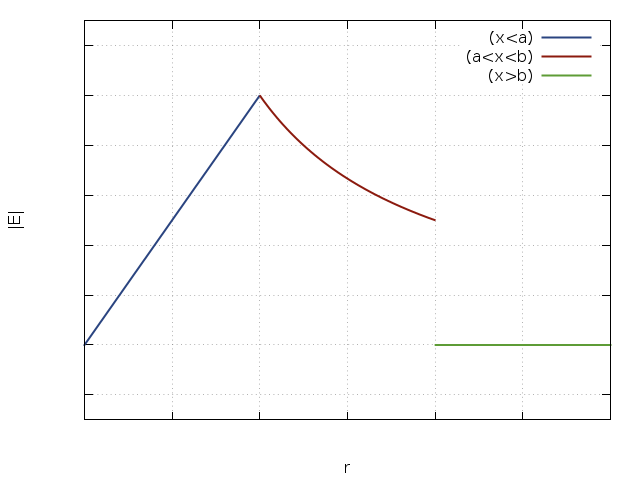
\includegraphics[scale=0.6]{Ex.png}
		%\caption{ $| \vec{E}(\vec{r}) |$ nas três regiões}
	\end{figure}
	
\end{document}
